\chapter{Opis projektnog zadatka}
		
	Cilj ovog projekta je razviti programsku podršku za web aplikaciju "Wild Track".
	Ta aplikacija olakšava korisniku pronalazak i praćenje divljih životinja.
	Prilikom otvaranja aplikacije prikazuje se karta koja pokazuje gdje se nalazi koja životinja.
	Praćene životinje imaju na sebi gps uređaj koji aplikaciji odašilje njihovu poziciju i tako korisnik može cijelo vrijeme znati njihovu točnu lokaciju.
	Kad korisnik odabere koju životinju želi pratiti, može vidjeti neke podatke o njoj, kao na primjer povijesne podatke gdje se nalazila, naziv vrste, slika i opis.
	
	Neregistrirani korisnik je ograničen samo s dosad nabrojanim akcijama, ako želi nešto više s aplikacijom omogućeno mu je prijavljivanje u sustav s postojećim računom 
	(potrebno je upisati korisničko ime i lozinku) ili kreiranjem novog računa. Za kreiranje novog računa potrebni su sljedeći podaci: 
	\begin{packed_item}
		\item uloga za koju se prijavljuje - može biti istraživač, voditelj postaje ili tragač na terenu
		\item korisničko ime 
		\item fotografija
		\item lozinka
		\item ime
		\item prezime
		\item email adresa
	\end{packed_item}

	Registracijom u sustav korisniku se dodjeljuju prava istraživača, voditelja postaje, tragača na terenu ili administratora.
	Registrirani korisnik može, uz opcije koje ima njegova željena uloga, još i pregledati, mijenjati osobne podatke te izbrisati svoj korisnički račun.

	Registracija je završena kad korisnik preko svoje email adrese potvrdi, osim ako je korisnik izabrao biti istraživač ili voditelj postaje. 
	U tom slučaju, administrator mora potvrditi njihovu ulogu. 
	Administrator sustava ima najveće ovlasti. 
	On ima ovlasti da vidi popis svih registriranih korisnika i njihovih osobnih podataka, odnosno pristup bazi s popisom registriranih korisnika, te može mijenjati njihova dodijeljena prava i osobne podatke.
	
	Voditelj postaje može izabrati koji će tragači biti dio njegove postaje i bira na koji način će oni izvoditi pretraživanje životinja. 
	Postaje su određena mjesta na karti koja voditelj postaje bira, to na primjer može biti postaja Biokovo ili postaja Lonjsko polje.

	Ako se korisnik prijavi kao tragač, njemu se na karti prikazuju zadaci koje mora obaviti, trenutna pozicija ostalih tragača koji su aktivni na istoj akciji, te trenutna pozicija životinja koje prate.
	Tragač tijekom svoje akcije može ostavljati komentare o životinji koju je pratio te također može ostaviti komentar ostalim tragačima i istraživačima, to jest drugim sudionicima u akciji.
	Također, cijeli put koji tragači prođu se bilježi, odnosno označavaju se staze kojima su putovali i način kojim su se kretali. To će biti potrebno istraživačima koji vizualiziraju njihovo kretanje u obliku toplinskih karata te potom to koriste za analiziranje kretanja životinja i njihovih omiljenih staništa.
	
	Načini kojima se tragači kreću mogu biti različiti, kao na primjer:
	\begin{packed_item}
		\item pješke
		\item dronom
		\item automobilom
		\item cross motorom
		\item brodom
		\item helikopterom
	\end{packed_item}

	Ovisno o tome kojom je tragač metodom osposobljen za obavljanje zadataka, svaka metoda je drugačije prikazana na karti.
	Svaka metoda pruža različitu vidljivost i područje pokrivanja te se na prikladne načine prikazuje na kartama. 
	Ako je tragač odabran da ide pješke njegova će karta biti detaljnija i prikazana na manjem prostoru nego karta tragača koji putuje helikopterom. 
	Tragači koji obavljaju zadatak s pomoću drona, helikoptera ili plovila, moraju na karti imati pravocrtnu rutu.
	Svaki tragač je osposobljen za samo jednu vozilo i tijekom te akcije se njegov tip prijevoza ne mijenja.

	Ako je korisnik odlučio biti istraživač, on može stvoriti nove akcije pretraživanja i praćenja životinja s detaljima o određenim vrstama, jedinkama ili staništima za proučavanje.
	Svaki istraživač je zadužen za jednu akciju.
	Ako je istraživaču potreban tragač za pomoć pri istraživanju, istraživač može poslati voditelju postaje zahtjev za tragačima s opisom o potrebnim kvalifikacijama.
	Voditelj će na taj zahtjev odabrati tragače koji odgovaraju opisu i postaviti ih da sudjeluju u toj akciji.
	Tragač će biti gotov s akcijom kad završi sve potrebne zadatke.
	Istraživač, kad dobije određene tragače, zadaje preko karte zadatke pojedinačno svakom tragaču.
	Zadaci mogu biti različiti, kao na primjer prolazak određenom rutom i dolazak do određene lokacije te postavljanje kamere ili uređaja za praćenje.
	Prilikom postavljanja zadatka, istraživač može i ostaviti neke dodatne komentare tragačima.
	Informacije o poziciji životinje, tragaču i postaji se istraživaču prikazuju preko interaktivne karte.
	Istraživač može birati da se tijekom izrade karte koriste i neke određene informacije. Na primjer:
	\begin{packed_item}
		\item povijesne pozicije praćenih životinja
		\item filtriranje životinja po vrsti ili pojedinačno po jedinki
		\item trenutne pozicije praćenih životinja
		\item povijesne pozicije svih tragača na nekoj akciji
		\item filtriranje po tipu prijevoza ili pojedinačno po tragaču
		\item trenutne pozicije tragača koji su aktivni na akciji
	\end{packed_item}


	

	Ovaj projekt može biti korisan svima koji bi htjeli više naučiti o divljim životinjama, ali isto tako i ljudima koji se bave proučavanjem životinja može olakšati posao.
	Svaka osoba koja želi može se ulogirati i postati tragač, u svrhu zabave, dodatnog znanja... A time, dok ljudi to rade iz zabave, odnosno svojevoljno, osobe koji su istraživači 
	mogu koristiti njihove informacije i time im se smanjuje dio posla.

	Slične aplikacije poput aplikacije "Wild Track" na području Hrvatske ne postoje. Neke aplikacije koje se bave divljim životinjama su: "eWildLife" i "Divlje životinje".

	"eWildLife" je aplikacija razvijena u realnom vremenu, ljudi prate i izvještavaju o ubijanju divljih životinja, 
	sukobe čovjek-životinja i viđenja divljih životinja, također mogu i spasiti delfine. 

	"Divlje životinje" (Slika \ref{fig:divlje_zivotinje}) je Android aplikacija koja omogućuje istraživanje svijeta životinja. 
	Aplikacija nudi opsežan katalog divljih životinja, uključujući šumske životinje, životinje iz zooloških vrtova, cirkuske životinje, afričke životinje, šumske životinje itd. 
	Aplikacija pruža detaljan opis svake životinje, uključujući njezinu vrstu, veličinu, kao i podatke o ponašanju i navikama. 
	Također možete pristupiti raznim slikama koje će vam pomoći da bolje razumijete životinje. 

	\begin{figure}[H]
		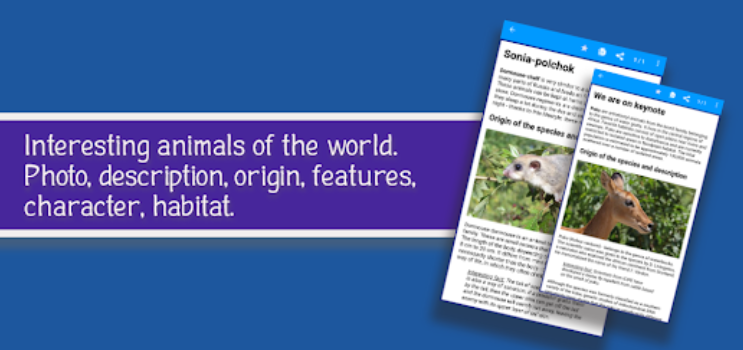
\includegraphics[scale=0.4]{slike/divlje_zivotinje.png} %veličina slike u odnosu na originalnu datoteku i pozicija slike
		\centering
		\caption{Aplikacija Divlje Životinje}
		\label{fig:divlje_zivotinje}
	\end{figure}

	No, slična aplikacija "Wild Track" aplikaciji izvan Hrvatske postoji. Zove se "Animal Tracker" (Slika \ref{fig:animal_tracker}). 
	S pomoću "Animal Tracker" aplikacije moguće je pratiti kretanje divljih životinja diljem svijeta koje se prate u gotovo stvarnom vremenu.
	Kretanja se prikupljaju GPS oznakama koje životinje nose i pohranjuju se u Movebank (internetska infrastruktura koju koriste istraživači za upravljanje, dijeljenje, analizu i arhiviranje podataka o kretanju životinja).


	\begin{figure}[H]
		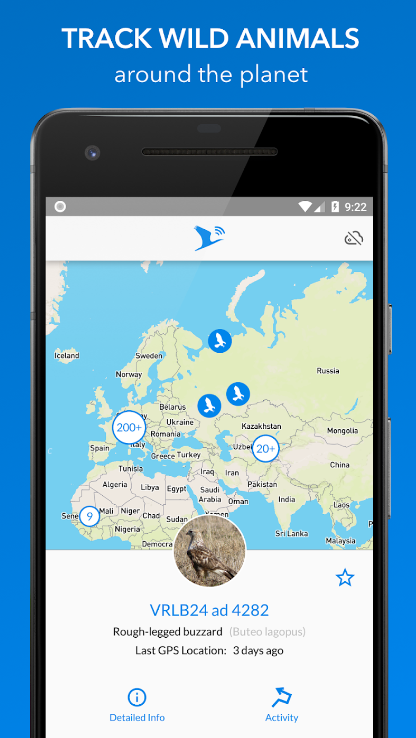
\includegraphics[scale=0.4]{slike/animal_tracker.png} %veličina slike u odnosu na originalnu datoteku i pozicija slike
		\centering
		\caption{Aplikacija Animal Tracker}
		\label{fig:animal_tracker}
	\end{figure}
	

	Poboljšanja na aplikacijama se uvijek mogu napraviti, pa tako može i na ovoj. Na primjer, moguće je pratiti otkucaje srca životinja, disanje\dots 
	Time je moguće određivati zdravlje životinje, kretnje životinje, da li životinja spava ili je budna\dots
	Tu smo dobili nove komponente aplikacije koje se mogu nazvati trenutne aktivnosti životinje i zdravlje životinje te tu tragači i istraživači imaju još više informacija o životinjama, a ne samo one općenite.
	Isto tako možemo dodati tragačima opciju da slikaju i snimaju životinje te im dati mogućnost da slike i videe objavljuju na aplikaciju. Time je opet doživljaj određene životinje bolji, a ne općenit.

	